\phantomsection
\appendix
\addcontentsline{toc}{section}{Anhang}

\begin{appendices}
\addtocontents{toc}{\protect\setcounter{tocdepth}{0}}


\section{Stichprobe}
\subsection{Soziodemografische Merkmale der Stichprobe}
\label{sec:appendix_demographics}

\begin{longtable}{p{5.5cm}p{5.5cm}rr}
    \caption{Übersicht über die Verteilung zentraler soziodemografischer Merkmale und Erfahrungen}
    \label{tab:soziodemografie_gesamt}\\
    \toprule
    Frage & Kategorie & Anzahl & Prozent \\
    \midrule
    \endfirsthead

    \multicolumn{4}{c}{{\bfseries Tabelle \thetable{} -- Fortsetzung}} \\
    \toprule
    Frage & Kategorie & Anzahl & Prozent \\
    \midrule
    \endhead
    
    \midrule
    \multicolumn{4}{r}{Fortsetzung auf der nächsten Seite}\\
    \endfoot
    
    \bottomrule
    \endlastfoot

    In welcher Altersgruppe befindest Du dich? & 16 – 25 & 20 & 80.0 \\*
     & 26 – 35 & 3 & 12.0 \\*
     & 56 – 65 & 1 & 4.0 \\*
     & Keine Angabe & 1 & 4.0 \\
    \midrule
    \addlinespace
    Welches Geschlecht wurde Dir bei der Geburt zugewiesen? & Männlich & 16 & 64.0 \\*
     & Weiblich & 8 & 32.0 \\*
     & Keine Angabe & 1 & 4.0 \\
    \midrule
    \addlinespace
    Mit welcher Geschlechtsidentität identifizierst Du dich? & Mann & 15 & 60.0 \\*
     & Frau & 9 & 36.0 \\*
     & Trans Mann & 1 & 4.0 \\
    \midrule
    \addlinespace
    Mit welchen Begriffen würdest du Deine sexuelle Orientierung beschreiben? & Heterosexuell & 17 & 68.0 \\*
     & Bisexuell & 3 & 12.0 \\*
     & Homosexual & 3 & 12.0 \\*
     & Queer & 1 & 4.0 \\*
     & Asexuell & 1 & 4.0 \\
    \midrule
    \addlinespace
    Was ist Dein höchster Bildungsabschluss? & Matura / Äquivalent & 23 & 92.0 \\*
     & Universitätsabschluss & 2 & 8.0 \\
    \midrule
    \addlinespace
    Wie ist Deine derzeitige berufliche oder schulische Situation? & Student\genderstern in / Schüler\genderstern in & 22 & 88.0 \\*
    & Angestellt & 3 & 12.0 \\
    \midrule
    \addlinespace
    Wie hoch ist ungefähr Euer gemeinsames monatliches Haushaltseinkommen (nach Abzug von Steuern)? & < CHF 1 500 & 7 & 28.0 \\*
     & CHF 1 500 – 3 000 & 2 & 8.0 \\*
     & CHF 3 000 – 4 500 & 2 & 8.0 \\*
     & CHF 6 000 – 7 500 & 2 & 8.0 \\*
     & CHF 7 500 – 10 000 & 1 & 4.0 \\*
     & > CHF 10 000 & 5 & 20.0 \\*
     & Nicht bekannt / bevorzugt nicht anzugeben & 6 & 24.0 \\
    \midrule
    \addlinespace
    Wie viele Personen leben in Deinem Haushalt (einschliesslich Dir selbst)? & 1 & 2 & 8.0 \\*
     & 2 & 3 & 12.0 \\*
     & 3 & 10 & 40.0 \\*
     & 4 & 6 & 24.0 \\*
     & 5 & 1 & 4.0 \\*
     & 6 & 2 & 8.0 \\*
     & 9 & 1 & 4.0 \\
    \midrule
    \addlinespace
    Wie viele Personen in Deinem Haushalt tragen (einschliesslich dir selbst) zum gemeinsamen Einkommen bei? & 1 & 6 & 24.0 \\*
     & 2 & 13 & 52.0 \\*
     & 3 & 4 & 16.0 \\*
     & 5 & 1 & 4.0 \\*
     & 6 & 1 & 4.0 \\
     \midrule
    \addlinespace
    Berechnetes Äquivalenz-Einkommen \parencite[nach][]{bundesamtfuerstatistikVerteilungVerfuegbarenAequivalenzeinkommens2025} & Armutsgefährdet & 8 & 32.0 \\*
     & Tief & 4 & 16.0 \\*
     & Mittel & 5 & 20.0 \\*
     & Hoch & 2 & 8.0 \\*
     & Unbekannt & 6 & 24.0 \\
     \midrule
    \addlinespace
    Hast Du eine körperliche oder psychische Beeinträchtigung, chronische Erkrankung oder andere gesundheitliche Einschränkung, die Deinen Alltag beeinflusst? & Nein & 25 & 100.0 \\
    \midrule
    \addlinespace
    Lebst Du in einem anderen Land, als in welchem du geboren wurdest? & Nein & 17 & 68.0 \\*
     & Ja & 7 & 28.0 \\*
     & Keine Angabe & 1 & 4.0 \\
     \midrule
    \addlinespace
    Hast Du im Alltag schon Diskriminierung aufgrund persönlicher Merkmale erlebt? & Ja, wegen meines Geschlechts & 4 & 16.0 \\*
     & Ja, wegen meiner Sprache oder meines Akzents & 4 & 16.0 \\*
     & Ja, wegen meiner Herkunft & 4 & 16.0 \\*
     & Ja, wegen meiner sexuellen Orientierung & 3 & 12.0 \\*
     & Ja, wegen meiner Kleidung oder meines Stils & 2 & 8.0 \\*
     & Ja, wegen meiner sozialen oder finanziellen Situation & 1 & 4.0 \\*
     & Ja, wegen meiner Hautfarbe oder meines Aussehens & 1 & 4.0 \\*
     & Ja, wegen meines Alters & 0 & 0.0 \\*
     & Ja, wegen meines Gesundheitszustands oder einer Behinderung & 0 & 0.0 \\*
     & Ja, aus einem anderen Grund & 0 & 0.0 \\*
     & Nein & 12 & 48.0 \\*
     & Keine Angabe & 0 & 0.0 \\
     \midrule
    \addlinespace
    Anzahl unterschiedlicher erlebter Diskriminierungsarten pro Person & 0 & 12 & 48.0 \\*
     & 1 & 8 & 32.0 \\*
     & 2 & 4 & 16.0 \\*
     & 3 & 1 & 4.0 \\
     \bottomrule
\end{longtable}

\clearpage
\subsection{Beschreibung der erfassten Momentaufnahmen}
\label{sec:appendix_moments}

\begin{longtable}{p{5.5cm}p{5.5cm}rr}
    \caption{Antworten auf die Fragen zu den Momentaufnahmen}
    \label{tab:moments}\\
    \toprule
    Frage & Kategorie & Anzahl & Prozent \\
    \midrule
    \endfirsthead

    \multicolumn{4}{c}{{\bfseries Tabelle \thetable{} -- Fortsetzung}} \\
    \toprule
    Frage & Kategorie & Anzahl & Prozent \\
    \midrule
    \endhead
    
    \midrule
    \multicolumn{4}{r}{Fortsetzung auf der nächsten Seite}\\
    \endfoot
    
    \bottomrule
    \endlastfoot

    Was machst Du gerade hauptsächlich? & Arbeiten oder studieren & 53 & 50.0 \\*
     & Freizeit oder Entspannung & 27 & 25.5 \\*
     & Unterwegs sein oder pendeln & 12 & 11.3 \\*
     & Kochen oder Essen & 8 & 7.5 \\*
     & Mediennutzung & 8 & 7.5 \\*
     & Soziale Aktivitäten & 7 & 6.6 \\*
     & Haushalt oder Aufräumen & 2 & 1.9 \\*
     & Ruhen / Schlafen & 2 & 1.9 \\*
     & Einkaufen oder Besorgungen & 2 & 1.9 \\*
     & Betreuungspflichten & 0 & 0.0 \\*
     & Sonstiges & 1 & 0.9 \\
    \midrule
    \addlinespace
    Bist Du drinnen oder draussen? & Drinnen & 54 & 50.9 \\*
     & Draussen & 52 & 49.1 \\
    \midrule
    \addlinespace
    Wo genau befindest Du dich? & Schule oder Universität & 38 & 35.8 \\*
     & Zuhause & 29 & 27.4 \\*
     & Unterwegs (zu Fuss, Fahrrad, Auto) & 12 & 11.3 \\*
     & Öffentlicher Verkehr & 8 & 7.5 \\*
     & Bei jemand anderem zuhause & 6 & 5.7 \\*
     & Arbeitsplatz & 5 & 4.7 \\*
     & Park oder Grünfläche & 5 & 4.7 \\*
     & Einkaufen oder Dienstleistungen & 2 & 1.9 \\*
     & Freizeit- oder Sporteinrichtung & 1 & 0.9 \\*
     & Café / Restaurant / Bar & 0 & 0.0 \\*
     & Kultureller oder religiöser Ort & 0 & 0.0 \\*
     & Gesundheitseinrichtung / Therapie & 0 & 0.0 \\*
     & Anderer Ort & 2 & 1.9 \\
     \midrule
    \addlinespace
    Mit wem bist Du gerade zusammen? & Freund\genderstern innen & 40 & 37.7 \\*
     & Allein & 38 & 35.8 \\*
     & Arbeitskolleg\genderstern innen & 17 & 16.0 \\*
     & Fremde & 17 & 16.0 \\*
     & Familie & 4 & 3.8 \\*
     & Bekannte & 3 & 2.8 \\*
     & Partner\genderstern in & 2 & 1.9 \\*
     & Tiere und Haustiere & 0 & 0.0 \\*
     & Kinder & 0 & 0.0 \\*
     & Andere & 2 & 1.9 \\
     \midrule
     \addlinespace
     Glaubst Du, dass dein Gefühl von Zugehörigkeit oder Fremdheit an diesem Ort damit zu tun hat, wie du als Person wahrgenommen wirst? & Nein & 58 & 54.7 \\*
     & Ja, wegen meines Alters & 17 & 16.0 \\*
     & Ja, wegen meiner Sprache oder meines Akzents & 17 & 16.0 \\*
     & Ja, wegen meiner sozialen oder finanziellen Situation & 15 & 14.2 \\*
     & Ja, wegen meiner Kleidung oder meines Stils & 13 & 12.3 \\*
     & Ja, wegen meiner Herkunft & 12 & 11.3 \\*
     & Ja, aus einem anderen Grund & 10 & 9.4 \\*
     & Ja, wegen meiner Hautfarbe oder meines Aussehens & 10 & 9.4 \\*
     & Ja, wegen meines Geschlechts & 9 & 8.5 \\*
     & Ja, wegen meines Gesundheitszustands oder einer Behinderung & 7 & 6.6 \\*
     & Ja, wegen meiner sexuellen Orientierung & 2 & 1.9 \\
     \midrule
     \addlinespace
     Verglichen mit den anderen Personen hier: Bei welchen Merkmalen fühlst Du dich der Mehrheit zugehörig? & In meinem Alter & 50 & 47.2 \\*
     & In meiner Sprache oder meines Akzents & 49 & 46.2 \\*
     & In meiner Hautfarbe oder meines Aussehens & 48 & 45.3 \\*
     & In meinem Gesundheitszustand oder einer Behinderung & 41 & 38.7 \\*
     & In meiner Herkunft & 37 & 34.9 \\*
     & In meiner sozialen oder finanziellen Situation & 37 & 34.9 \\*
     & In meiner Kleidung oder meines Stils & 34 & 32.1 \\*
     & In meinem Geschlecht & 27 & 25.5 \\*
     & In meiner sexuellen Orientierung & 22 & 20.8 \\*
     & Ich bin alleine hier & 22 & 20.8 \\
     \bottomrule
\end{longtable}


\begin{figure}[htbp]
    \centering
    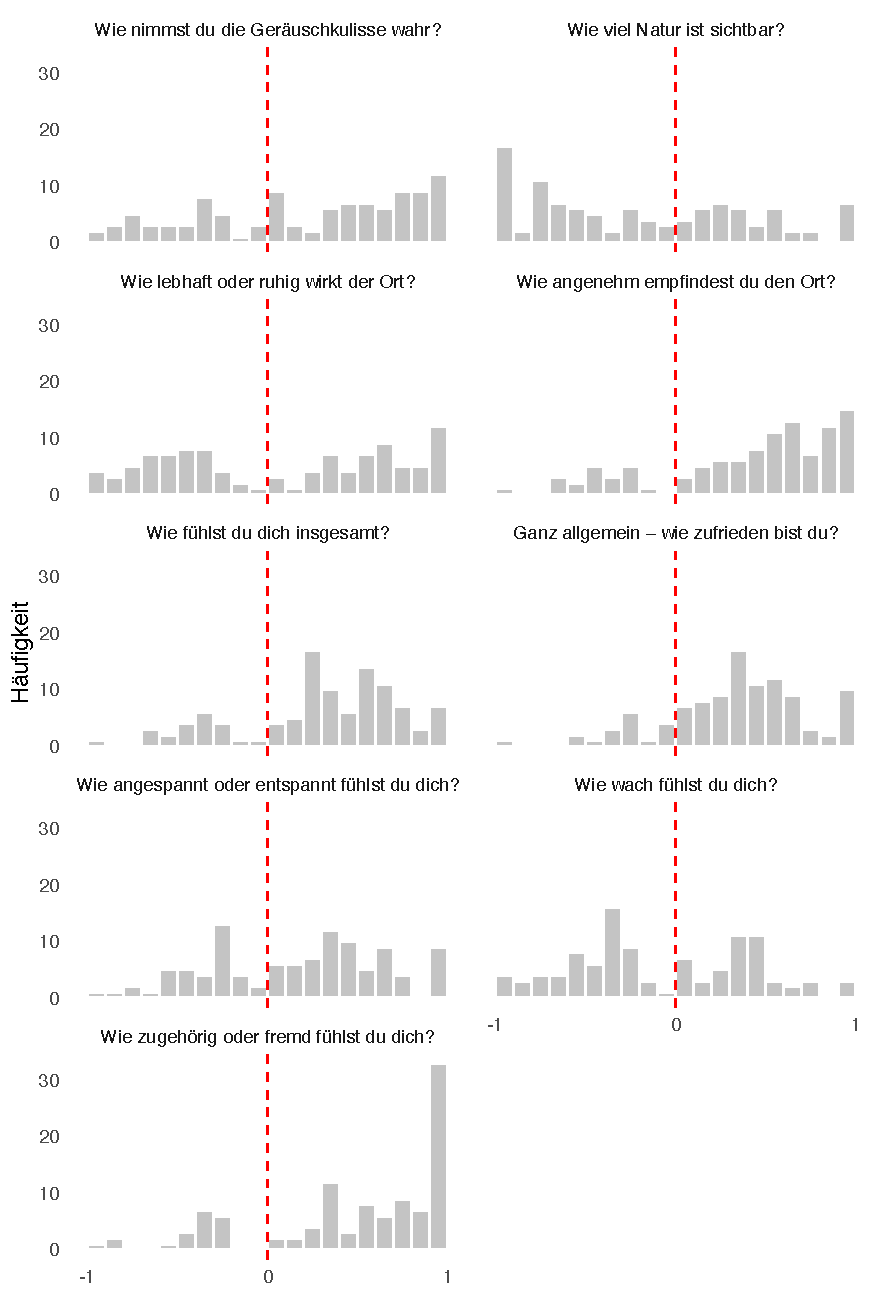
\includegraphics[width=\textwidth]{analysis/plots/slider_hists.pdf}
    \caption{Histogramme der Slider-Items}
    \label{fig:slider_hists}
\end{figure}

\begin{longtable}{p{5.5cm}p{9.5cm}}
    \caption{Antworten auf Freitextfragen}
    \label{tab:freitext}\\
    \toprule
    Frage & Antwort \\
    \midrule
    \endfirsthead

    \multicolumn{2}{c}{{\bfseries Tabelle \thetable{} -- Fortsetzung}} \\
    \toprule
    Frage & Antwort \\
    \midrule
    \endhead
    
    \midrule
    \multicolumn{2}{r}{Fortsetzung auf der nächsten Seite}\\
    \endfoot
    
    \bottomrule
    \endlastfoot

    Gibt es andere Dinge die dazu führen, dass Du dich hier weniger wohl oder unwohl fühlst? & heat \\*
     & Everyone is doing the same, so it kind of feels like being at the right place \\*
     & The contact with strangers \\*
     & Bed \\*
     & health issues \\*
     & no natural sunlight room without windows no fresh air \\*
     & a lot of people - personal space \\*
     & No \\*
     & / \\*
     & no \\*
     & Not really \\
    \midrule
    \addlinespace
    Gibt es andere Dinge die dazu führen, dass Du dich hier wohler fühlst? & place i know and is mine i have control over it \\*
     & know this place and can do what i want \\*
     & my room and cozy for the night \\*
     & pets \\*
     & spending time with family pets \\*
     & I am not by myself \\*
     & Less noise from construction works \\
    \bottomrule
\end{longtable}


\addtocontents{toc}{\protect\setcounter{tocdepth}{2}}

\end{appendices}